\documentclass[a4paper, 11pt]{article}

\usepackage[utf8x]{inputenc}
\usepackage[T1]{fontenc}
\usepackage{ucs}
\usepackage[english]{babel}
\usepackage{mathtools}
\usepackage{amsmath}
\usepackage{amsfonts}
\usepackage{ulem}
\usepackage{verbatim}
\usepackage{fancyhdr}
\usepackage[parfill]{parskip}
\usepackage{graphicx}
\usepackage{palatino}
\usepackage{float}
\usepackage[font={small,it}]{caption}

\linespread{1.05}
\pagestyle{fancyplain}
\fancyhead{}
\fancyfoot[L]{}
\fancyfoot[C]{}
\fancyfoot[R]{\thepage}
\renewcommand{\headrulewidth}{0pt}
\renewcommand{\footrulewidth}{0pt}
\setlength{\headheight}{13.6pt}

\widowpenalty=1000
\clubpenalty=1000

\newcommand{\horrule}[1]{\rule{\linewidth}{#1}}

\title{ 
\normalfont \normalsize 
\textsc{University of Copenhagen} \\ [25pt]
\horrule{0.5pt} \\[0.4cm]
\huge PCSD: Assignment 2 \\
\horrule{2pt} \\[0.5cm]
}

\author{Jens Fredskov (chw752)\\Henrik Bendt (gwk553)\\Ronni Lindsgaard (mxb392)} % Your name

\date{\normalsize\today} % Today's date or a custom date

\begin{document}
\maketitle
\pagebreak

\section{Serializability \& Locking}
The predecence graph for Schedule 1 can be seen in figure \ref{fig:schedule1}.
As there is a cycle the schedule is not conflict-serializable. The schedule
could not have been generated using strict two-phase locking as the write to X
in T2 needs to happen after the read in T1. T1 cannot be completed and thus
releasing the lock of X as T3 needs to release the read lock for Y. T3 cannot
run before T2 which is visible in the predence graph. 

\begin{figure}[H]
  \centering
  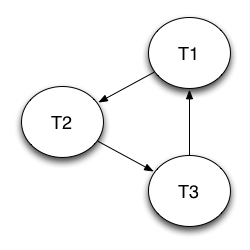
\includegraphics[width=0.5\textwidth]{images/schedule1}
  \caption{Precedence graph for Schedule 1. The cycle shows that the schedule is
  not conflict-serializable.}
  \label{fig:schedule1}
\end{figure}


Figure \ref{fig:schedule2} show the precedence graph for Schedule 2. There is no
cycle which means it is conflict serializable. Figure \ref{fig:schedule2-2pl}
shows injected read/write locks in accordance with strict 2PL rules.
 
\begin{figure}[H]
  \centering
  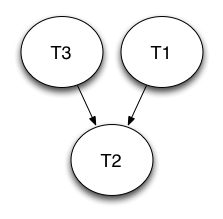
\includegraphics[width=0.5\textwidth]{images/schedule2}
  \footnotesize
  \caption{Precedence graph for Schedule 2. The absence of a cycle show that the
  schedule is conflict-serializable.}
  \label{fig:schedule2}
\end{figure}

\begin{figure}[H]
\footnotesize
\centering
\verbatiminput{figures/schedule2-2pl.txt}
\caption{Schedule 2 with read- (RL) and writelocks (WL) induced. All locks are
released on commits. The unlock operations are omitted for simplicity of the
table.}
\label{fig:schedule2-2pl}
\end{figure}


\section{Optimistic Concurrency Control} % (fold)
\label{sec:optimistic_concurrency_control}

\paragraph{Scenario 1} % (fold)
\label{par:scenario_1}

Here test 2 applies, but as the intersection of the write set for T2 and the read set for T3 equals $\{4\}$, T3 is not allowed to commit and must roll back.

% paragraph scenario_1 (end)

\paragraph{Scenario 2} % (fold)
\label{par:scenario_2}

Here test 2 applies, but as the intersection of the write set for T1 and the read set for T3 equals $\{3\}$, T3 is not allowed to commit and must roll back. 

% paragraph scenario_2 (end)

\paragraph{Scenario 3} % (fold)
\label{par:scenario_3}

Here test 2 applies both between T1/T3 and T2/T3. As both tests pass T3 is allowed to commit.

% paragraph scenario_3 (end)

% section optimistic_concurrency_control (end)

\end{document}

